%{

{
\cleardoublepage

%\pagestyle{plain}      % ← отключаем fancy-стиль
%\thispagestyle{plain}  % ← на текущей (первой) странице эпилога

\phantomsection

\fancyhead[LE]{\fancyplain{}{}}
\fancyhead[RO]{\fancyplain{}{}}

%\pagestyle{empty}
%\thispagestyle{mystyle}
%\addtocontents{toc}{\vspace{-5mm}}
\bookmarksetup{startatroot}% this is it
%\addtocontents{toc}{\vspace{1\baselineskip}}
\addcontentsline{toc}{chapter}{Эпилог}
%\pdfbookmark[-1]{Эпилог}{epilog}
%\addtocontents{toc}{\vspace{-6mm}}
\section*{Эпилог}
%\chapter*{Эпилог}

%Перевалило за полночь. Шурик сидел у себя на~кухне в~домашних штанах и майке, лениво потягивая из коньячного бокала 7\sdash летний ром. Жена у плиты хлопотала блинчики сыну на утро. Шурик задумчиво рассматривал жену сзади, любуясь, будто бы в первый раз, формами. Их сын мирно посапывал в кроватке. В мире творился трындец. Жизнь~продолжалась$\ldots$

Перевалило за полночь. Шурик сидел у себя на~кухне в~домашних штанах и майке, лениво потягивая из коньячного бокала. Жена у плиты хлопотала блинчики сыну на утро. Шурик задумчиво рассматривал жену сзади, любуясь, будто бы в первый раз, формами. Их сын мирно посапывал в~кроватке. 

Никаких его проблем сплав, поход, конечно же не~решил, да и не мог решить. Но отдых, тем не менее, удался на славу\mdash это Шурик мог утверждать с уверенностью. Они оторвались с пацанами по полной программе, б\'{о}льшего и~желать грешновато на одно путешествие двухнедельное\mdash и в Старой Ладоге побывали, и на Киваче, и пороги взяли, и~поробинзонили, и рыбы наелись карельской, наговорились обо всём, напитались атмосферой Карелии.

Это путешествие, как и любой другой их вояж по~рекам, выключило команду из привычного опостылевшего ритма городской жизни и заставило пережить бурю ярких эмоций и~гамму чувств. Это ли не смысл отдыха? Смена деятельности, порой такая вот <<ударная>>. Мышцы рук к~концу похода уже полностью адаптировались и перестали ныть от весла, втянулись, что называется. Тут бы плыть и~плыть, ан нет, пожалуйте обратно в <<каменные джунгли>>.

Жена что\sdash то говорила ему, он на автомате отвечал, а~всеми мыслями был ещё там, на реке. Там он был Адмиралом, где под его началом Команда проходила Маршрут, где он решал в каком месте вставать лагерем, 

В мире творился трындец. Жизнь~продолжалась$\ldots$

sedfslidgfdj spofk opfk sepspo sefrs posdfps pos sedfslidgfdj spofk opfk sepspo sefrs posdfps pos sedfslidgfdj spofk opfk sepspo sefrs posdfps pos sedfslidgfdj spofk opfk sepspo sefrs posdfps pos sedfslidgfdj spofk opfk sepspo sefrs posdfps pos sedfslidgfdj spofk opfk sepspo sefrs posdfps pos sedfslidgfdj spofk opfk sepspo sefrs posdfps pos sedfslidgfdj spofk opfk sepspo sefrs posdfps pos sedfslidgfdj spofk opfk sepspo sefrs posdfps pos sedfslidgfdj spofk opfk sepspo sefrs posdfps pos sedfslidgfdj spofk opfk sepspo sefrs posdfps pos sedfslidgfdj spofk opfk sepspo sefrs posdfps pos sedfslidgfdj spofk opfk sepspo sefrs posdfps pos sedfslidgfdj spofk opfk sepspo sefrs posdfps pos sedfslidgfdj spofk opfk sepspo sefrs posdfps pos sedfslidgfdj spofk opfk sepspo sefrs posdfps pos sedfslidgfdj spofk opfk sepspo sefrs posdfps pos sedfslidgfdj spofk opfk sepspo sefrs posdfps pos sedfslidgfdj spofk opfk sepspo sefrs posdfps pos sedfslidgfdj spofk opfk sepspo sefrs posdfps pos sedfslidgfdj spofk opfk sepspo sefrs posdfps pos sedfslidgfdj spofk opfk sepspo sefrs posdfps pos sedfslidgfdj spofk opfk sepspo sefrs posdfps pos sedfslidgfdj spofk opfk sepspo sefrs posdfps pos sedfslidgfdj spofk opfk sepspo sefrs posdfps pos sedfslidgfdj spofk opfk sepspo sefrs posdfps pos sedfslidgfdj spofk opfk sepspo sefrs posdfps pos 

%Надпись:

%{\centering\Large{\fontspec{NorseRus}{%
%	Текст текст текст\\
%}}}
%
%Карелия$\ldots$

%}%

\begin{center}
	\psvectorian[scale=0.4]{88} % Красивый вензелёк :)
\end{center}

\begin{center}
	\Large {КОНЕЦ}
\end{center}
}

%\vspace*{\fill}
\vspace{2cm}
\begin{flushright}
	\copyright~Соболев~А.А.,~Москва,~\today\\
%	\copyright~Соболев~А.А.,~Москва,~01.01.1970\\
%	\textit{ред.~01.01.1970}
\end{flushright}

%}

%\vspace{5mm}
%\begin{flushright}
%\textit{Соболев А.А., 2023 г.}
%%\copyright~Соболев~А.А.,~Москва,~27.08.2015
%\end{flushright}

%\pagestyle{plain}

%\newpage
%\clearpage
%\pagestyle{plain}

%\clearpage
%\thispagestyle{plain}  % ← чтобы и картинка была без колонтитулов

\phantomsection

\fancyhead[LE]{\fancyplain{}{}}
\fancyhead[RO]{\fancyplain{}{}}

\vspace*{4.0em}

%\vspace*{\fill}
%\begin{wrapfigure}[18]{l}{0.5\textwidth}
\begin{figure}[!h]
	\centering
	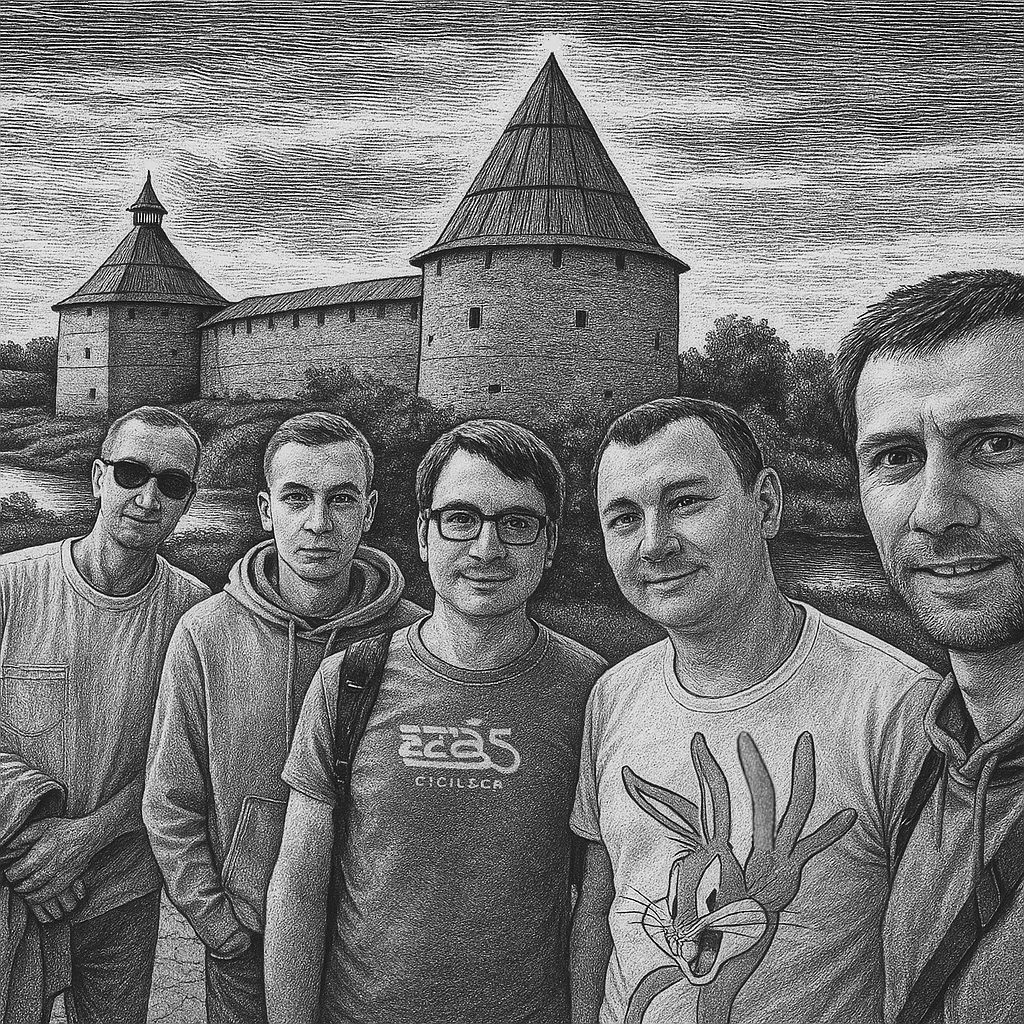
\includegraphics[width=1.0\textwidth]{60_komanda}
%	\caption{\small\textit{...упиваясь красотой местных пейзажей...}}
\end{figure}
%\end{wrapfigure}
%\vspace*{\fill}


%}

%}